\section{范畴与\trSimplicialSet{}}
\label{sec:categories-and-simplicial-sets}

本节旨在让读者熟悉我们全书要研究的基本对象：\trSimplicialSet{}。看待%
\trSimplicialSet{}最自然的方式，是把它当作单纯指标范畴（simplicial indexing
category）$\Delta$ 上的\trPresheaf{}（presheaf）范畴，而 $\Delta$ 我们马上就会定义。随后
我们将研习（普通）范畴论中的若干基本概念，并讨论由\trNerve{}（nerve）构造所实现的%
\trSimplicialSet{}与普通\trCategory{}之间的关系；这条构造断言：范畴构成的范畴到%
\trSimplicialSet{}中的嵌入是\trFullyFaithful{}，而且人们可以显式刻画哪些%
\trSimplicialSet{}作为\trCategory{}的\trNerve{}出现。
为了回避谈论类，我们将在一个集合论框架下工作，此框架马上介绍。除了通常的 ZFC
公理（即 Zermelo--Fraenkel 集合论再加上选择公理）之外，我们还假设一条额外的公
理，称为大基数公理：

\begin{axiom*}
对每个基数 $\kappa$，都存在一个不可达基数 $\kappa'$，使得
$\kappa' > \kappa$。
\end{axiom*}

若由遗传基数小于 $\kappa$ 的那些集合组成的集族 $\mathcal{V}_{<\kappa}$（即该集
合与其所有成员的基数都小于 $\kappa$）自身满足 ZFC 公理，则称基数 $\kappa$ 为不可
达的（inaccessible）。集族 $\mathcal{V}_{<\kappa}$ 称为一个宇宙（universe）。事实
表明，这条大基数公理无法从 ZFC 证出，而且实际上它在逻辑上独立。特别地，不可达基
数 $\kappa$ 大于任何 $\aleph_k$。由这条公理，我们可以取定一列不可达基数
\[
\kappa_0 < \kappa_1 < \kappa_2 < \dots
\]
并考虑与之相伴的诸宇宙 $\mathcal{V}_{<\kappa}$。

\begin{definition}\label{def:small-large-very-large-sets}
称一个集合为
\begin{enumerate}[label=(\arabic*)]
  \item 小的，若它包含于 $\mathcal{V}_{<\kappa_0}$；
  \item 大的，若它包含于 $\mathcal{V}_{<\kappa_1}$；
  \item 很大的，若它包含于 $\mathcal{V}_{\kappa_2}$；\footnote{译注：原书此处印作
  $\mathcal{V}_{\kappa_2}$，按体例疑脱「$<$」。}
  \item 非常非常大的，若它包含于 $\mathcal{V}_{<\kappa_3}$，依此类推。
\end{enumerate}
在本书中，除小、大与很大的集合之外，我们不会遇到任何别的集合。
\end{definition}

\begin{example*}
由所有小集合构成的集合是大的；由所有大集合构成的集合是
很大的，如此等等。
\end{example*}

\begin{definition}\label{def:category}
一个\trCategory{} $\mathcal{C}$ 由下述数据组成：一个（可能大的）对象集
$\mathrm{ob}(\mathcal{C})$，以及对任意两个对象 $x$、$y$，一个（同样可能大的）态射
集 $\mathrm{Hom}_{\mathcal{C}}(x,y)$，并配备合成映射
\[
\mathrm{Hom}_{\mathcal{C}}(x,y) \times \mathrm{Hom}_{\mathcal{C}}(y,z) \to
\mathrm{Hom}_{\mathcal{C}}(x,z)
\]
与单位元 $* \to \mathrm{Hom}_{\mathcal{C}}(x,x)$（对所有对象 $x$），且满足结合律与
单位性。

称一个\trCategory{}为\emph{局部小的}（locally small），若所有态射集
$\mathrm{Hom}_{\mathcal{C}}(x,y)$ 都是小的；称它为\emph{小的}，若它局部小而且对象
集也是小的；称它为\emph{本质小的}（essentially small），若它局部小而且对象的同构
类之集是小的。
\end{definition}

\begin{remark}\label{rem:locally-small}
在范畴论中，\trCategory{}通常定义成具有一个（可能是真）类的对象，并且对任意两个
对象具有一个由态射构成的集合。用我们的语言说，这就是我们所称的局部小范畴。然而一
般而言，我们并不假设\trCategory{}是局部小的。
\end{remark}

\begin{definition}\label{def:poset}
一个偏序集（partially ordered set）是一个集合 $P$，配备了一个自反、反对称且传递的
关系 $\le$。也就是说：$a \le a$；若 $a \le b$ 且 $b \le a$，则 $a = b$；若
$a \le b$ 且 $b \le c$，则 $a \le c$。偏序集之间的映射是满足如下条件的集合映射
$f\colon P \to Q$：$x \le y$ 蕴含 $f(x) \le f(y)$。这就定义了一个范畴
$\mathrm{PoSet}$，其对象为偏序集，其态射为偏序集的映射。
\end{definition}

\begin{example*}
\emph{有限线性序集：}集合 $\{0,1,\dots,n\}$ 上有线性序
$0 \le 1 \le \dotsb \le n$，记作 $[n]$。一个一般的有限偏序集 $S$ 称为线性序的，若
它同构于某个 $[n]$。线性序集的态射就是底偏序集的态射。这样我们得到一个范畴
$\mathrm{LinOrdSet}$。
\end{example*}

\begin{example*}
\emph{子集偏序集：}设 $S$ 是一个集合，考虑它的子集之集
$\mathcal{P}(S)$：$\mathcal{P}(S) = \{\, I \subseteq S \,\}$。这个集合按包含关系
成为一个偏序集：
\[
I \le J \iff I \subseteq J
\]
\end{example*}

\begin{definition}\label{def:delta}
范畴 $\Delta$ 是偏序集范畴 $\mathrm{PoSet}$ 中由对所有 $n \ge 0$ 的线性序集
$[n]$ 组成的满子范畴。注意，从 $[n]$ 到 $[m]$ 的态射因此就恰是弱单调映射。
\end{definition}

\begin{example*}
$\Delta$ 中有两类特殊的映射，即\trFaceMap{}（face map）与\trDegeneracyMap{}（degeneracy map）。对每
个 $n \ge 0$ 与 $0 \le i \le n$，\trFaceMap{}是映射
\[
d_i\colon [n-1] \to [n]
\]
它由性质 $i \notin \mathrm{Im}(d_i)$ 以及 $d_i$ 为单射唯一确定。此外，对 $n \ge 1$
与 $0 \le i \le n-1$，\trDegeneracyMap{}是映射
\[
s_i\colon [n] \to [n-1]
\]
它们由性质 $|s_i^{-1}(i)| = 2$ 以及 $s_i$ 为满射唯一确定。换言之，我们有
$s_i(i) = s_i(i+1) = i$。
\end{example*}

\begin{definition}\label{def:presheaf}
设 $\mathcal{C}$ 是一个\trCategory{}。我们把由\trFunctor{} $\mathcal{C}^{\mathrm{op}} \to \mathrm{Set}$ 构成的\trCategory{}记作 $\mathcal{P}(\mathcal{C})$，并称之为
$\mathcal{C}$ 上的\trPresheaf{}范畴。对象 $x \in \mathcal{C}$ 确定一个\emph{可表的}\trPresheaf{}%
（representable presheaf），即\trPresheaf{} $\mathrm{Hom}_{\mathcal{C}}(-,x)$，它把
$y \in \mathcal{C}$ 送到从 $y$ 到 $x$ 的态射之集。这就确定了一个\trFunctor{}%
$\mathcal{C} \to \mathcal{P}(\mathcal{C})$，称为\emph{\trYoneda{}嵌入}（Yoneda
embedding）。
\end{definition}

\begin{definition}\label{def:simplicial-set}
一个\trSimplicialSet{}是 $\Delta$ 上的一个\trPresheaf{}，即一个\trFunctor{}%
$\Delta^{\mathrm{op}} \to \mathrm{Set}$。给定\trSimplicialSet{} $X$，它的
$n$-\trSimplex{}之集由 $X([n])$ 给出，并将记作 $X_n$。称一个 $n$-\trSimplex{} $x$ 为\emph{退化的}，
如果存在满射 $\alpha\colon [n] \to [m]$（其中 $m \neq n$）与某个 $n$-\trSimplex{} $y$ 使得
$x = \alpha^*(y)$。等价地，若 $x = s_i^*(y)$，其中 $y \in X_{n-1}$ 且
$0 \le i \le n-1$，则 $x$ 退化。称一个 $n$-\trSimplex{}为\emph{非退化的}，如果它不退化。
我们把\trSimplicialSet{}的\trCategory{} $\mathcal{P}(\Delta)$ 记作
$\mathrm{sSet}$。
\end{definition}

\begin{definition}\label{def:standard-simplex}
令 $\Delta^n$ 表示由 $[n] \in \Delta$ 所表示的\trSimplicialSet{}。具体地，我们有
$(\Delta^n)_m = \mathrm{Hom}_{\Delta}([m],[n])$。
\end{definition}

\begin{definition}\label{def:pi0}
设 $X$ 是一个\trSimplicialSet{}。考虑 $0$-\trSimplex{}之集 $X_0$ 上由如下规定生成的等价关
系 $\sim$：若存在 $1$-\trSimplex{} $f \in X_1$ 使得 $d_0(f) = x$ 且 $d_1(f) = y$，则将 $x$
与 $y$ 相关联。（这个关系是自反的，但一般既不传递也不对称。）于是我们如下定义集合
$\pi^{\Delta}_0(X)$：
\[
\pi^{\Delta}_0(X) = X_0 / {\sim}
\]
\end{definition}

\begin{lemma}\label{lem:yoneda-lemma}
\trYoneda{}引理：设 $F\colon \mathcal{C}^{\mathrm{op}} \to \mathrm{Set}$ 是一个\trFunctor{}，
$x \in \mathcal{C}$ 是一个对象。那么映射
\[
\mathrm{Hom}_{\mathcal{P}(\mathcal{C})}\bigl(\mathrm{Hom}_{\mathcal{C}}(-,x),
F\bigr) \to F(x)
\]
（由把 $\eta$ 送到 $\eta(\mathrm{id}_x)$ 给出）是一个双射。
\end{lemma}
\begin{proof}
其逆由把元素 $s \in F(x)$ 送到函数 $\mathrm{Hom}_{\mathcal{C}}(y,x) \to F(y)$（把
$f$ 送到 $f^*(s)$）给出。可以直接验证这是一个\trNaturalTransformation{}，而且是上
述映射的逆。
\end{proof}

\begin{lemma}\label{lem:yoneda-embedding-fully-faithful}
\trYoneda{}嵌入 $\mathcal{C} \to \mathcal{P}(\mathcal{C})$ 是\trFullyFaithful{}。
\end{lemma}

\begin{proof}
这由\trYoneda{}引理立即得出：\trYoneda{}嵌入在态射上的作用是映射
\[
\mathrm{Hom}_{\mathcal{C}}(x,y) \to
\mathrm{Hom}_{\mathcal{P}(\mathcal{C})}\bigl(\mathrm{Hom}_{\mathcal{C}}(-,x),
\mathrm{Hom}_{\mathcal{C}}(-,y)\bigr)
\]
它由把 $f$ 送到
\[
\mathrm{Hom}_{\mathcal{C}}(z,x) \xrightarrow{\ f_*\ }
\mathrm{Hom}_{\mathcal{C}}(z,y)
\]
给出。易见这个映射与\trYoneda{}引理中描述的那个映射互逆；后者把态射
$f \in \mathrm{Hom}_{\mathcal{C}}(x,y)$ 送到函数 $\mathrm{Hom}_{\mathcal{C}}(z,x) \to \mathrm{Hom}_{\mathcal{C}}(z,y)$，其把 $\varphi$ 送到 $\varphi^*(f) = f_*\varphi$。
\end{proof}

\begin{corollary}\label{cor:hom-delta-n-x}
对\trSimplicialSet{} $X$，存在典范双射
\[
\mathrm{Hom}_{\mathrm{sSet}}(\Delta^n, X) \cong X_n.
\]
\end{corollary}

\begin{definition}\label{def:colimit}
\trFunctor{} $F\colon I \to \mathcal{C}$ 的一个（余）\trLimit{}是 $\mathcal{C}$ 的一个对
象，简记作 $\operatorname{colim}_I F$，并配有映射 $F(i) \to \operatorname{colim}_I F$（对每个 $i \in I$）；这些映射按如下意义相容：对 $I$ 中每个态射 $i \to j$，图表
\begin{center}
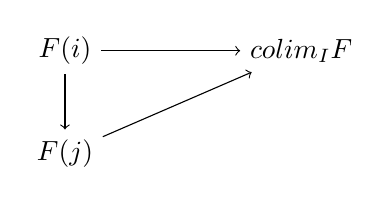
\begin{tikzpicture}
  \node (fi) at (0,0) {$F(i)$};
  \node (cl) at (3,0) {$\operatorname{colim}_I F$};
  \node (fj) at (0,-1.3) {$F(j)$};
  \draw[->] (fi) -- (cl);
  \draw[->] (fi) -- (fj);
  \draw[->] (fj) -- (cl);
\end{tikzpicture}
\end{center}
交换。这个数据要求满足下述泛性质：每当再给定一个对象 $X \in \mathcal{C}$，它也配备
有按上述方式相容的映射 $F(i) \to X$，则存在唯一的态射 $\operatorname{colim}_I F \to X$ 使得图表
\begin{center}
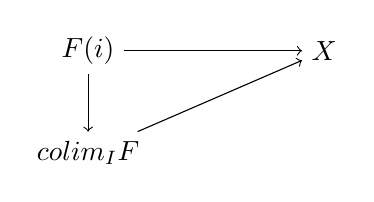
\begin{tikzpicture}
  \node (fi) at (0,0) {$F(i)$};
  \node (x) at (3,0) {$X$};
  \node (cl) at (0,-1.3) {$\operatorname{colim}_I F$};
  \draw[->] (fi) -- (x);
  \draw[->] (fi) -- (cl);
  \draw[->] (cl) -- (x);
\end{tikzpicture}
\end{center}
交换。对偶地，$F$ 的一个\trLimit{}是对象 $\operatorname{lim}_I F$，配有映射
$\operatorname{lim}_I F \to F(i)$，它们同样相容，并满足对偶的泛性质：每当给定一个
对象 $X$，配有对所有 $i \in I$ 的相容态射 $X \to F(i)$，则存在唯一的态射
$X \to \operatorname{lim}_I F$ 使显然的图表交换。
\end{definition}

\begin{remark}\label{rem:universal-property-unique-iso}
注意，这样的泛性质在唯一同构的意义下确定一个对象。还要注意，泛性质所涉及的不仅仅
是对象 $\operatorname{colim}_I F$ 本身：那些参照映射是数据的一部分，而正是这一点使
得对象在唯一同构的意义下唯一。
\end{remark}

\begin{example*}
空图表 $\varnothing \to \mathcal{C}$ 的\trColimit{}是一
个\trInitialObject{}，即一个到任何其他对象均有唯一态射的对象。对偶地，空图表
$\varnothing \to \mathcal{C}$ 的\trLimit{}是一个\trTerminalObject{}，即一个从任何
其他对象均有唯一态射而来的对象。
\end{example*}

\begin{example*}
定义在图表 $\bullet \leftarrow \bullet \rightarrow \bullet$
上的\trFunctor{}的\trColimit{}称为\emph{\trPushout{}}（pushout）。对偶地，定义在图表
$\bullet \rightarrow \bullet \leftarrow \bullet$ 上的\trFunctor{}的\trLimit{}称为\emph{\trPullback{}}
（pullback）。
\end{example*}

\begin{example*}
商向量空间 $V/U$ 是图表
\begin{center}
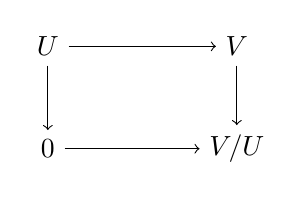
\begin{tikzpicture}
  \node (u) at (0,0) {$U$};
  \node (v) at (2.4,0) {$V$};
  \node (z) at (0,-1.3) {$0$};
  \node (q) at (2.4,-1.3) {$V/U$};
  \draw[->] (u) -- (v);
  \draw[->] (u) -- (z);
  \draw[->] (z) -- (q);
  \draw[->] (v) -- (q);
\end{tikzpicture}
\end{center}
的一个\trPushout{}。
\end{example*}

\begin{observation}\label{obs:colimits-via-initial-terminal}
人们可以把一般的（余）\trLimit{}通过\trInitialObject{}与\trTerminalObject{}来表述
。当我们在\trInfinityCategories{}中讨论\trLimit{}与\trColimit{}时，将会用到这一观
点。给定一个\trFunctor{}%
$F\colon I \to \mathcal{C}$，我们可以考虑这个\trFunctor{}的（余）锥范畴。给定\trCategory{}%
$I$，我们考虑两个新范畴 $I^{\lhd}$ 与 $I^{\rhd}$，它们由 $I$ 分
别添入一个\trInitialObject{}相应地一个\trTerminalObject{}而得到。有显然的\trFunctor{}%
$I \to I^{\lhd}$ 与 $I \to I^{\rhd}$。于是我们可以考虑\trFunctor{}范畴
$\mathrm{Fun}_F(I^{\lhd}, \mathcal{C})$ 与 $\mathrm{Fun}_F(I^{\rhd}, \mathcal{C})$，
即沿上述包含限制到 $F$ 的那些\trFunctor{}构成的范畴。它们分别称为 $F$ 上方的
锥范畴与余锥范畴。于是可以证明：如上描述的\trColimit{}是余锥范畴中的一个%
\trInitialObject{}，而\trLimit{}是锥范畴中的一个\trTerminalObject{}。\footnote{译注：原书此处两句互换（作「余极限……锥范畴……始对象」「极限……余锥范畴……终对象」），与其前对锥范畴（$\mathrm{Fun}_F(I^{\lhd},\mathcal{C})$）与余锥范畴（$\mathrm{Fun}_F(I^{\rhd},\mathcal{C})$）的划分不合，据其自定义径改。——译者注}
\end{observation}

下述引理由（余）极限的定义以及\cref{ex:set-bicomplete} 中建立的事实（范畴 $\mathrm{Set}$ 是\trBicomplete{}的
）立即得出（否则该陈述根本没有意义）。

\begin{lemma}\label{lem:hom-out-of-colimit}
设 $\mathcal{C}$ 是一个\trCategory{}，$F\colon I \to \mathcal{C}$ 是 $\mathcal{C}$
中一个 $I$ 形图表。那么对每个对象 $x \in \mathcal{C}$，存在典范双射
\begin{enumerate}[label=(\arabic*)]
  \item $\mathrm{Hom}_{\mathcal{C}}(\operatorname{colim}_I F, x) \cong \operatorname{lim}_I \mathrm{Hom}_{\mathcal{C}}(F(i), x)$，且
  \item $\mathrm{Hom}_{\mathcal{C}}(x, \operatorname{lim}_I F) \cong \operatorname{lim}_I \mathrm{Hom}_{\mathcal{C}}(x, F(i))$。
\end{enumerate}
此外，这些双射唯一地刻画（余）\trLimit{}。
\end{lemma}

\begin{definition}\label{def:adjunction}
一个\emph{\trAdjunction{}}由一对\trFunctor{} $(F\colon \mathcal{C} \to \mathcal{D},\, G\colon \mathcal{D} \to \mathcal{C})$ 连同一个自然同构组成；该自然同构介于两个\trFunctor{}%
$\mathcal{C}^{\mathrm{op}} \times \mathcal{D} \to \mathrm{Set}$ 之间：
\[
\mathrm{Hom}_{\mathcal{D}}(F(-),-)
\qquad\text{与}\qquad
\mathrm{Hom}_{\mathcal{C}}(-,G(-)).
\]
\end{definition}

给定\trFunctor{} $F\colon \mathcal{C} \to \mathcal{D}$ 与图表 $X\colon I \to \mathcal{C}$，
存在典范比较映射
\[
\operatorname{colim}_I F(X) \longrightarrow F(\operatorname{colim}_I X)
\qquad\text{相应地}\qquad
F(\operatorname{lim}_I X) \longrightarrow \operatorname{lim}_I F(X).
\]
若相应的比较映射是同构，则称 $F$ 保持余极限，相应地保持极限。

\begin{lemma}\label{lem:adjoints-preserve}
\trLeftAdjoint{}保持余极限，而\trRightAdjoint{}保持极限。
\end{lemma}
\begin{proof}
设 $F\colon \mathcal{C} \to \mathcal{D}$ 是一个容有\trRightAdjoint{}（设为 $G$）的\trFunctor{}，
并设 $X\colon I \to \mathcal{C}$ 是一个有\trColimit{}%
$\operatorname{colim}_I X \in \mathcal{C}$ 的图表。我们断言：$F$ 把这个余极限送到图
表 $I \to \mathcal{C} \to \mathcal{D}$ 的一个余极限。用公式说，我们断言：由相容映射
$F(X(i)) \to F(\operatorname{colim}_I X(i))$——它们是余极限数据的一部分，然后再应用
$F$——所诱导的典范映射 $\operatorname{colim}_I F(X(i)) \to F(\operatorname{colim}_I X(i))$
是同构。为看清这一点，只需证明该典范映射对所有其他对象 $y \in \mathcal{D}$
在态射集上诱导双射：
\begin{align*}
\mathrm{Hom}_{\mathcal{D}}(F(\operatorname{colim}_I X(i)), y)
&\cong \mathrm{Hom}_{\mathcal{C}}(\operatorname{colim}_I X(i), Gy) \\
&\cong \operatorname{lim}_I \mathrm{Hom}_{\mathcal{C}}(X(i), Gy) \\
&\cong \operatorname{lim}_I \mathrm{Hom}_{\mathcal{D}}(F(X(i)), y) \\
&\cong \mathrm{Hom}_{\mathcal{D}}(\operatorname{colim}_I F(X(i)), y)
\end{align*}
由\trYoneda{}引理，证明即告完成。关于\trRightAdjoint{}保持极限的断言，论证类似。
\end{proof}

\begin{lemma}\label{lem:adjoint-unique}
设 $F\colon \mathcal{C} \to \mathcal{D}$ 是容有\trRightAdjoint{} $G$ 与 $G'$ 的\trFunctor{}。
那么在 $G$ 与 $G'$ 之间存在一个被指明的自然同构，它由「与诸伴随相容」这一条件唯
一刻画。因此，伴随\trFunctor{}若存在，则在唯一同构的意义下唯一。
\end{lemma}

\begin{proof}
考虑如下两个自然双射：
\[
\mathrm{Hom}_{\mathcal{C}}(Gx, G'x) \cong
\mathrm{Hom}_{\mathcal{D}}(FGx, x) \cong
\mathrm{Hom}_{\mathcal{C}}(Gx, Gx)
\]
那么 $Gx$ 的恒等映射便对应到一个自然变换 $G \to G'$。对
$\mathrm{Hom}_{\mathcal{C}}(G'x, Gx)$ 施行同样的技巧，即可看出这必是一个自然同构。
\end{proof}

\begin{definition}\label{def:bicomplete}
称一个\trCategory{}为（余）完备的，如果它容有以任意小\trCategory{}为指标的（余）
\trLimit{}。\footnote{译注：原书此处括注「(statt (co)limits)」，其中 statt 为德语
（意为「而非」），疑为排印疏漏。}若它既完备又余完备，则称它为\trBicomplete{}的。
\end{definition}

\begin{lemma}\label{lem:colimit-adjoint-constant}
若 $\mathcal{C}$ \trBicomplete{}，则（余）\trLimit{}构造与常值图表\trFunctor{}互为左／右伴随。特别
地，构造（余）\trLimit{}确定了一个\trFunctor{}%
\[
\mathrm{Fun}(I, \mathcal{C}) \to \mathcal{C}.
\]
\end{lemma}
\begin{proof}
我们把余极限的情形详细写出。考虑常值\trFunctor{} $\mathrm{const}\colon \mathcal{C} \to \mathrm{Fun}(I,\mathcal{C})$。
现在为每个\trFunctor{} $F\colon I \to \mathcal{C}$ 指定一个对
象，即 $\operatorname{colim}_I F$。\trColimit{}数据的一部分是相容映射族
$\{\, F(i) \to \operatorname{colim}_I F \,\}_{i \in I}$，它们显然能拼装成一个%
\trNaturalTransformation{}%
\[
F \to \operatorname{const}(\operatorname{colim}_I F).
\]
接着，我们考虑复合
\[
\begin{aligned}
\mathrm{Hom}_{\mathcal{C}}(\operatorname{colim}_I F, X) &\to
\mathrm{Hom}_{\mathrm{Fun}(I,\mathcal{C})}\bigl(\operatorname{const}
(\operatorname{colim}_I F), \operatorname{const} X\bigr) \\
&\to
\mathrm{Hom}_{\mathrm{Fun}(I,\mathcal{C})}(F, \operatorname{const} X)
\end{aligned}
\]
由\trColimit{}的泛性质，它是双射。于是本引理由\cref{ex:adjoint-via-hom-bijection} 即得。极限的情形完全类似。
\end{proof}

\begin{lemma}\label{lem:post-composition-adjoint}
给定一个\trAdjunction{}，其中 $F\colon \mathcal{C} \to \mathcal{D}$ 是
$G\colon \mathcal{D} \to \mathcal{C}$ 的左伴随；再给定一个辅助的小\trCategory{}%
$I$，则诸\trFunctor{}%
\[
F_*\colon \mathrm{Fun}(I,\mathcal{C})
\rightleftarrows \mathrm{Fun}(I,\mathcal{D})\colon G_*
\]
仍构成一个伴随对。这里 $F_*$ 由与 $F$ 作后合成给出，同样地，$G_*$ 由与 $G$ 作后合成
给出。
\end{lemma}

\begin{proof}
该\trAdjunction{}由一个余单位映射 $\varepsilon\colon FG \to \mathrm{id}_{\mathcal{D}}$
与一个单位映射 $\eta\colon \mathrm{id}_{\mathcal{C}} \to GF$ 确定，二者满足\cref{ex:adjunction-unit-counit} 的
三角恒等式。现在我们用这些映射为\trFunctor{}对 $(F_*, G_*)$ 构造余单位映射与单位映射如下：
设 $\varphi \in \mathrm{Fun}(I,\mathcal{D})$。我们需要为\trFunctor{} $I \to \mathcal{D}$ 指
定一个自然映射 $\varepsilon_*\colon F_*(G_*(\varphi)) \to \varphi$；设
$x \in \mathcal{E}$。\footnote{译注：原书此处作「$x \in \mathcal{E}$」，但
$\mathcal{E}$ 从未定义；按上下文（$\varepsilon_*$ 的分量以 $x$ 标号、需代入
$\varphi(x)$，而 $\varphi\colon I \to \mathcal{D}$）应为 $I$。}我们把新的余单位 $\varepsilon_*$
定义为映射
\[
F(G(\varphi(x))) \xrightarrow{\ \varepsilon_{\varphi(x)}\ } \varphi(x).
\]
由于 $\varepsilon$ 本身是一个\trNaturalTransformation{}，容易看出这在 $\varphi$ 上
是自然的。类似地，我们定义\trNaturalTransformation{}%
$\eta_*\colon \psi \to G_*F_*(\psi)$ 为
\[
\psi(y) \xrightarrow{\ \eta_{\psi(y)}\ } G(F(\psi(y))).
\]
于是容易看出三角恒等式成立，因为 $(\varepsilon, \eta)$ 满足三角恒等式。
\end{proof}
\begin{proposition}\label{prop:functor-category-bicomplete}
若 $\mathcal{C}$ 是\trBicomplete{}\trCategory{}，则 $\mathrm{Fun}(I,\mathcal{C})$ 也是\trBicomplete{}的。
图表 $X\colon J \to \mathrm{Fun}(I,\mathcal{C})$ 的一个（余）\trLimit{}由把
$i \in I$ 送到 $\operatorname{colim}_J X(j)(i)$ 的那个\trFunctor{}给出。
\end{proposition}

\begin{proof}
我们来证明 $\mathrm{Fun}(I,\mathcal{C})$ 是余完备的。完备性的论证类似（或者可以通
过正确地应用\trFunctor{} $(-)^{\mathrm{op}}$ 从这一情形形式地推出）。我们断言，复合
\[
\mathrm{Fun}(J,\mathrm{Fun}(I,\mathcal{C})) \cong
\mathrm{Fun}(I,\mathrm{Fun}(J,\mathcal{C}))
\xrightarrow{\ \operatorname{colim}_J\ }
\mathrm{Fun}(I,\mathcal{C})
\]
就是我们要证其存在的那个余极限\trFunctor{}。由\cref{lem:post-composition-adjoint}，这个\trFunctor{}%
有一个\trRightAdjoint{}，由
\[
\mathrm{const}_*\colon \mathrm{Fun}(I,\mathcal{C}) \to
\mathrm{Fun}(I,\mathrm{Fun}(J,\mathcal{C})) \cong
\mathrm{Fun}(J,\mathrm{Fun}(I,\mathcal{C}))
\]
给出。一旦我们确认这个\trFunctor{}本身是常值\trFunctor{}（由定义立即可得），命题便得证，因为那时我
们可以援引\cref{lem:colimit-adjoint-constant}。
\end{proof}

\begin{corollary}\label{cor:sset-bicomplete}
\trSimplicialSet{}的\trCategory{} $\mathrm{sSet}$ 是\trBicomplete{}的。
\end{corollary}

\begin{definition}\label{def:slice-category}
设 $\mathcal{D}$ 是一个\trCategory{}，$x$ 是 $\mathcal{D}$ 的一个对象。\trSliceCategory{}%
$\mathcal{D}_{/x}$ 的对象是诸对 $(d \in \mathcal{D},\ \alpha\colon d \to x)$；从
$(d,\alpha)$ 到 $(d',\alpha')$ 的态射由 $\mathcal{D}$ 中那些使涉及 $\alpha$、
$\alpha'$ 与 $\beta$ 的显然三角形交换的映射 $\beta\colon d \to d'$ 组成。有一个典范\trFunctor{}%
$\mathcal{D}_{/x} \to \mathcal{D}$，它把对 $(d,\alpha)$ 送到 $d$。
若 $F\colon \mathcal{C} \to \mathcal{D}$ 是一个\trFunctor{}，且 $x \in \mathcal{D}$ 是一个对
象，我们用\trPullback{}定义由 $F$ 与 $x$ 确定的\trSliceCategory{}：
\begin{center}
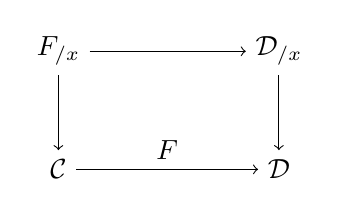
\begin{tikzpicture}
  \node (fx) at (0,0) {$F_{/x}$};
  \node (dx) at (2.8,0) {$\mathcal{D}_{/x}$};
  \node (c) at (0,-1.5) {$\mathcal{C}$};
  \node (d) at (2.8,-1.5) {$\mathcal{D}$};
  \draw[->] (fx) -- (dx);
  \draw[->] (fx) -- (c);
  \draw[->] (c) -- node[above] {$F$} (d);
  \draw[->] (dx) -- (d);
\end{tikzpicture}
\end{center}
于是 $F_{/x}$ 的对象是诸对 $(c \in \mathcal{C},\ \alpha\colon F(c) \to x)$，其态射由
那些使涉及 $\alpha$、$\alpha'$ 与 $F(\beta)$ 的显然三角形交换的映射
$\beta\colon c \to c'$ 组成。
有时，特别是当 $F$ 是一个子范畴的包含\trFunctor{}时，我们干脆写 $\mathcal{C}_{/x}$ 来代替
$F_{/x}$，而让\trFunctor{} $F$ 不言自明。还有一个显然对偶的\trSliceCategory{}概念，由
$\mathcal{D}_{x/}$ 构造，其对象是诸对 $(d,\ \alpha\colon x \to d)$。在下文中，我们
使用与\cref{def:presheaf}中\trYoneda{}嵌入 $\mathcal{C} \to \mathcal{P}(\mathcal{C})$
相关联的\trSliceCategory{}。
\end{definition}

\begin{lemma}\label{lem:presheaf-colimit-representables}
{\sloppy\hbadness=5000
每个\trPresheaf{}都是若干可表\trObject{}的\trColimit{}。更精确地说，对每个%
\trPresheaf{}%
$F\colon \mathcal{C}^{\mathrm{op}} \to \mathrm{Set}$，自明映射（tautological map）
\[
\operatorname*{colim}_{X \in \mathcal{C}_{/F}}
\mathrm{Hom}_{\mathcal{C}}(-,X) \to F
\]
是同构。\par}
\end{lemma}

\begin{proof}
证明再次依赖\trYoneda{}引理，也就是说，我们要证该映射对到任一辅助\trPresheaf{} $G$ 的映射诱
导双射。为此我们计算
\begin{align*}
\mathrm{Hom}_{\mathcal{P}(\mathcal{C})}\Bigl(
\operatorname*{colim}_{X \in \mathcal{C}_{/F}}
\mathrm{Hom}_{\mathcal{C}}(-,X),\, G\Bigr)
&\cong \operatorname*{lim}_{X \in \mathcal{C}_{/F}}
\mathrm{Hom}_{\mathcal{P}(\mathcal{C})}\bigl(\mathrm{Hom}_{\mathcal{C}}(-,X),\,
G\bigr) \\
&\cong \operatorname*{lim}_{X \in \mathcal{C}_{/F}} G(X).
\end{align*}
不难看出，最后一项其实就是从 $F$ 到 $G$ 的\trNaturalTransformation{}之集。
\end{proof}

设 $i\colon \mathcal{C}_0 \subseteq \mathcal{C}$ 是一个\trCategory{}的小子范畴，并
设 $\mathcal{D}$ 是一个\trBicomplete{}\trCategory{}。

\begin{fact}\label{fact:restriction-adjoints}
限制\trFunctor{}%
\[
i^*\colon \mathrm{Fun}(\mathcal{C},\mathcal{D}) \to
\mathrm{Fun}(\mathcal{C}_0,\mathcal{D})
\]
有一个左伴随，记作 $i_!$；还有一个右伴随，记作 $i_*$。它们由
\[
i_!(F)(x) = \operatorname*{colim}_{c \in (\mathcal{C}_0)_{/x}} F(c)
\]
与
\[
i_*(F)(y) = \operatorname*{lim}_{c \in (\mathcal{C}_0)_{x/}} F(x)
\]
给出。\footnote{译注：原书后一公式如此印出；按上下文（右\trKanExtension{}的标准公式）应
为 $\operatorname*{lim}_{c \in (\mathcal{C}_0)_{y/}} F(c)$。}
注意，按假设这些切片都是小的，因此上式中的余极限与极限均存在。让自己确信这套公式确
实给出限制\trFunctor{} $i^*$ 的伴随，是一个不错的练习。
\end{fact}

\begin{definition}\label{def:kan-extension}
在上述情形中，我们称 $i_!(F)$ 为 $F$ 沿 $i$ 的\emph{左\trKanExtension{}}（left Kan
extension），称 $i_*(F)$ 为 $F$ 沿 $i$ 的\emph{右\trKanExtension{}}（right Kan
extension）。
\end{definition}

\begin{observation}\label{obs:identity-kan-extension}
「自明映射是同构」这一陈述表明：$\mathcal{P}(\mathcal{C})$ 的恒等\trFunctor{}是\trYoneda{}%
嵌入的一个左\trKanExtension{}（沿\trYoneda{}嵌入）。
\end{observation}

\begin{corollary}\label{cor:colim-preserving-restriction-equivalence}
若 $\mathcal{D}$ 是余完备\trCategory{}，而 $\mathcal{C}$ 是小\trCategory{}，则沿%
\trYoneda{}嵌入限制所得的典范\trFunctor{}%
\[
\mathrm{Fun}^{\mathrm{colim}}(\mathcal{P}(\mathcal{C}), \mathcal{D}) \to
\mathrm{Fun}(\mathcal{C},\mathcal{D})
\]
是一个\trEquivalence{}。这里 $\mathrm{Fun}^{\mathrm{colim}}$ 记\trFunctor{}范畴中由保持余极
限的那些\trFunctor{}组成的满子范畴。
\end{corollary}

\begin{proof}
给定\trFunctor{} $f\colon \mathcal{C} \to \mathcal{D}$，我们想构造一个保持余极限的\trFunctor{}%
$\hat{f}\colon \mathcal{P}(\mathcal{C}) \to \mathcal{D}$，使得对 $X \in \mathcal{C}$
有 $\hat{f}(X) = f(X)$。由\cref{lem:presheaf-colimit-representables}，给定对象
$F \in \mathcal{P}(\mathcal{C})$，我们不得不定义
\[
\hat{f}(F) = \operatorname*{colim}_{X \in \mathcal{C}_{/F}} f(X).
\]
容易验证这确实是一个\trFunctor{}：对 $\mathcal{P}(\mathcal{C})$ 中的态射 $F \to G$，用所给态
射作后合成便诱导一个从范畴 $\mathcal{C}_{/F}$ 到范畴 $\mathcal{C}_{/G}$ 的\trFunctor{}；于是
不难看出，取余极限会产生一个映射
\[
\operatorname*{colim}_{X \in \mathcal{C}_{/F}} f(X) \to
\operatorname*{colim}_{X \in \mathcal{C}_{/G}} f(X).
\]
同样可以很快看出，这确实是一个\trFunctor{}。
为了看出这个\trFunctor{}保持余极限，我们注意到 $\hat{f}$ 容有一个右伴随 $G$，由
\[
G(d)(X) = \mathrm{Hom}_{\mathcal{D}}(f(X), d)
\]
给出。
在\cref{lem:presheaf-colimit-representables}的证明中我们看到，$F$ 与 $F'$ 之间的%
\trNaturalTransformation{}之集由
\[
\mathrm{Hom}_{\mathcal{P}(\mathcal{C})}(F, F') =
\operatorname*{lim}_{X \in \mathcal{C}_{/F}} F'(X)
\]
给出。因此我们看到
\[
\mathrm{Hom}_{\mathcal{D}}\bigl(\hat{f}(F), d\bigr) \cong
\operatorname*{lim}_{X \in \mathcal{C}_{/F}}
\mathrm{Hom}_{\mathcal{D}}(f(X), d) \cong
\operatorname*{lim}_{X \in \mathcal{C}_{/F}} G(d)(X).
\]
于是 $\hat{f}$ 是 $G$ 的左伴随，从而保持余极限。
\end{proof}

\begin{corollary}\label{cor:sset-colimit-representables}
设 $X$ 是一个\trSimplicialSet{}。那么
\[
X \cong \operatorname*{colim}_{[n] \in \Delta_{/X}} \Delta^n.
\]
\end{corollary}

\begin{lemma}\label{lem:internal-hom-adjoint}
设 $X$ 是一个固定的\trSimplicialSet{}。那么把 $Y$ 送到 $X \times Y$ 的\trFunctor{}%
$\mathrm{sSet} \to \mathrm{sSet}$ 容有一个右伴随 $\underline{\mathrm{Hom}}(X,-)$，它
由公式
\[
\mathrm{Hom}_{\mathrm{sSet}}\bigl(\Delta^n,
\underline{\mathrm{Hom}}(X,Z)\bigr) =
\mathrm{Hom}_{\mathrm{sSet}}(\Delta^n \times X, Z)
\]
确定。有时我们也把 $\underline{\mathrm{Hom}}(X,Z)$ 写作 $Z^X$。
\end{lemma}

\begin{proof}
把 $[n]$ 送到右端那个集合，显然确定了一个\trSimplicialSet{}，我们称之为
$\underline{\mathrm{Hom}}(X,Z)$。由于它在可表\trSimplicialSet{}上满足伴随性质，我
们可以把这个伴随扩张到所有\trSimplicialSet{}上。（记住：每个\trSimplicialSet{}都是
可表对象的余极限。）注意，我们用到了 $X \times -\colon \mathrm{sSet} \to \mathrm{sSet}$
保持余极限这一事实。这在 $\mathrm{Set}$ 中肯定成立，因为态射集提供了
一个右伴随。
\end{proof}

\begin{definition}\label{def:top}
我们令 $\mathrm{Top}$ 为对象是拓扑空间、态射是连续映射的\trCategory{}。下列对象对我
们很重要：设 $n \ge 0$ 是一个自然数。拓扑 $n$-\trSimplex{} $\Delta^n_{\mathrm{top}}$ 是
$\R^{n+1}_{\ge 0}$ 中由坐标之和为 $1$ 的那些点构成的子空间。拓扑\trSimplex{}构成一个
\emph{余单纯}空间 $[n] \mapsto \Delta^n_{\mathrm{top}}$，其中诸诱导映射是唯一的仿射
线性映射，它们在顶点上的行为恰如所需。
更精确地说，给定 $\alpha\colon [n] \to [m]$，诱导映射
$\alpha_*\colon \Delta^n_{\mathrm{top}} \to \Delta^m_{\mathrm{top}}$ 由
\[
\alpha_*(t_0, \dots, t_n) = (v_0, \dots, v_m)
\]
给出，其中 $v_i = \sum_{j \to i} t_j$。
\end{definition}

\begin{definition}\label{def:singular-simplicial-set}
一个拓扑空间 $X$ 的\emph{\trSingularSimplicialSet{}}（singular simplicial set）是\trSimplicialSet{}%
\[
\mathcal{S}(X) = \bigl([n] \mapsto
\mathrm{Hom}_{\mathrm{Top}}(\Delta^n_{\mathrm{top}}, X)\bigr).
\]
\end{definition}

\begin{definition}\label{def:geometric-realization}
\trGeometricRealization{} $|-|\colon \mathrm{sSet} \to \mathrm{Top}$ 是唯一一个保持余极限并把
$\Delta^n$ 送到 $\Delta^n_{\mathrm{top}}$ 的\trFunctor{}。具体地，\trSimplicialSet{} $X$ 的%
\trGeometricRealization{}是拓扑空间
\[
|X| = \operatorname*{colim}_{\Delta^n \in \Delta_{/X}} \Delta^n_{\mathrm{top}}.
\]
一个更为具体的公式是
\[
|X| = \Bigl( \coprod_{n \in \Delta} X_n \times \Delta^n_{\mathrm{top}} \Bigr)
\big/ \bigl( (f^*(x),\, t) \sim (x,\, f_*(t)) \bigr)
\]
其中 $x \in X_n$，$t \in \Delta^m_{\mathrm{top}}$，而 $f\colon [m] \to [n]$ 是
$\Delta$ 中的一个态射。
\end{definition}

\begin{proposition}\label{prop:singular-right-adjoint}
奇异复形是\trGeometricRealization{}的右伴随。
\end{proposition}

\begin{proof}
按伴随的定义，我们需要为\trFunctor{} $\mathrm{sSet}^{\mathrm{op}} \times \mathrm{Top} \to \mathrm{Set}$
指定一个自然同构，它介于
\[
\mathrm{Hom}_{\mathrm{Top}}(|X|, Y)
\qquad\text{与}\qquad
\mathrm{Hom}_{\mathrm{sSet}}(X, \mathcal{S}(Y))
\]
之间。但由前面的工作我们知道，这两个\trFunctor{}等价于
\[
\operatorname*{lim}_{\Delta/X} \mathrm{Hom}_{\mathrm{Top}}(\Delta^n_{\mathrm{top}},
Y)
\qquad\text{与}\qquad
\operatorname*{lim}_{\Delta/X} \mathrm{Hom}_{\mathrm{sSet}}(\Delta^n,
\mathcal{S}(Y)),
\]
而在取极限之前，后两者就已经（按 $\mathcal{S}(Y)$ 的定义）同构了。
\end{proof}
\begin{definition}\label{def:boundary-horn-spine}
\begin{enumerate}[label=(\arabic*)]
  \item 边缘 $\partial\Delta^n$ 是 $\Delta^n$ 的子单纯集，其 $k$-\trSimplex{}由非满射的映射
  $[k] \to [n]$ 组成。
  \item 对任意子集 $S \subseteq [n]$，$S$-\trHorn{} $\Lambda^n_S \subseteq \Delta^n$
  由那些 $k$-\trSimplex{} $f\colon [k] \to [n]$ 组成，使得存在 $i \in [n] \setminus S$ 不在
  $f$ 的像之中。一个\trHorn{} $\Lambda^n_j = \Lambda^n_{\{j\}}$ 称为\emph{内%
  \trHorn{}}（inner horn），如果 $0 < j < n$；称它为（左或右）\emph{外\trHorn{}}
  （outer horn），如果 $j = 0$ 相应地 $j = n$。
  \item \emph{\trSpine{}}（spine）$I^n \subseteq \Delta^n$ 由那些 $k$-\trSimplex{}%
  $f\colon [k] \to [n]$ 给出，其像集形如 $\{j\}$ 或 $\{j, j+1\}$。
\end{enumerate}
\end{definition}

\begin{definition}\label{def:skeleton-coskeleton}
\trSimplicialSet{} $X$ 的 $n$-\trSkeleton{} $\mathrm{sk}_n(X)$ 由\trSimplicialSet{}%
$i_!i^*(X)$ 给出，其中 $i\colon \Delta_{\le n} \subseteq \Delta$ 是由基数 $\le n+1$
的那些对象组成的满子范畴的包含。对偶地，\trSimplicialSet{}的 $n$-余\trSkeleton{}%
$\mathrm{cosk}_n(X)$ 由\trSimplicialSet{} $i_*i^*(X)$ 给出。这蕴含
$\mathrm{cosk}_n(X)$ 的 $k$-\trSimplex{}由
\[
\mathrm{cosk}_n(X)_k = \mathrm{Hom}_{\mathrm{sSet}}(\mathrm{sk}_n(\Delta^k), X)
\]
给出。
\end{definition}

\begin{lemma}\label{lem:skeleton-coskeleton-adjoint}
\begin{enumerate}[label=(\arabic*)]
  \item \trSkeleton{} $\mathrm{sk}_n(X)$ 同构于 $X$ 的最小子单纯集，后者的 $k$-\trSimplex{}之集在
  $k \le n$ 时与 $X$ 的相合。
  \item \trFunctor{} $\mathrm{sk}_n$ 与 $\mathrm{cosk}_n$ 互为左、右伴随。
  \item 有公式 $\mathrm{cosk}_n(X) = \mathrm{Hom}_{\mathrm{sSet}}(\mathrm{sk}_n(\Delta^{\bullet}), X)$。
\end{enumerate}
\end{lemma}

\begin{proof}
\begin{enumerate}[label=(\arabic*)]
  \item 易见映射 $\mathrm{sk}_n(X) \to X$ 逐层单射，且对 $k \le n$ 有
  $\mathrm{sk}_n(X)_k = X_k$。给定任何其他具有此性质的子单纯集 $Z$，我们有
  $\mathrm{sk}_n(X) = \mathrm{sk}_n(Z) \subseteq Z$，断言得证。
  \item 显然，因为伴随可以复合。
  \item 显然，由 (2)。
\end{enumerate}
\end{proof}

\begin{lemma}\label{lem:realization-horn-spine}
\trHorn{}的\trGeometricRealization{}是一个\trHorn{}，而\trSpine{}的\trGeometricRealization{}是一条\trSpine{}。
\end{lemma}
\begin{proof}
这由 $|\Delta^n| = \Delta^n_{\mathrm{top}}$ 这一事实以及下述观察得出：
\begin{enumerate}[label=(\arabic*)]
  \item $I^n = I^{n-1} \coprod_{\Delta^0} \Delta^1$；
  \item 存在余等化子
\[
\coprod_{0 \le i \le j \le n} \Delta^{[n]\setminus i} \times_{\Delta^n}
\Delta^{[n]\setminus j}
\;\Longrightarrow\;
\coprod_{0 \le i \le n,\; i \neq k} \Delta^{[n]\setminus i}
\;\longrightarrow\;
\Lambda^n_i.
\]
\footnote{译注：原书如此——下标 $k$ 未曾定义，末项 $\Lambda^n_i$ 疑应为 $\Lambda^n_j$。}
\end{enumerate}
\end{proof}

\begin{corollary}\label{cor:realization-cw-complex}
\trSimplicialSet{}的\trGeometricRealization{}是 \trCWComplex{}。
\end{corollary}

\begin{proof}
给定\trSimplicialSet{} $X$，通过 $|\mathrm{sk}_n(X)| \subseteq |X|$ 在 $|X|$ 上定义一
个过滤。由于\trGeometricRealization{}与余极限交换，我们看到这确实构成 $|X|$ 的一个过滤，而上述的那些%
\trPushout{}给出\trGeometricRealization{}的\trPushout{}。接着我们用到 $|\partial\Delta^n| \cong S^{n-1}$ 与
$|\Delta^n| \cong D^n$。
\end{proof}

\begin{observation}\label{obs:poset-to-category}
一个偏序集按如下方式确定一个\trCategory{}：对象是偏序集 $P$ 的元素，且对每对元素
$x, y \in P$，我们有
\[
\mathrm{Hom}(x, y) =
\begin{cases}
* & \text{若 } x \le y, \\
\varnothing & \text{否则。}
\end{cases}
\]
此外，与偏序集相伴的\trCategory{}之间的\trFunctor{}无非是偏序集的映射，即尊重偏序的
集合映射。这就确定了一个\trFullyFaithful{}\trFunctor{} $\mathrm{PoSet} \to \mathrm{Cat}$。
由此我们可以把 $[n]$ 视作一个\trCategory{}。把 $[n]$ 送到这个范畴，便得到一个余单纯
小\trCategory{}。
\end{observation}

\begin{definition}\label{def:nerve}
\trCategory{} $\mathcal{C}$ 的\trNerve{}是由
\[
[n] \mapsto \mathrm{Fun}([n], \mathcal{C}),
\]
给出的\trSimplicialSet{}；也就是说，它是通过从上述余单纯\trCategory{}到给定%
\trCategory{}取\trFunctor{}而得到的。
\end{definition}
\begin{lemma}\label{lem:delta-n-nerve}
$\Delta^n$ 同构于\trCategory{} $[n]$ 的\trNerve{}。
\end{lemma}

\begin{proof}
展开定义，我们发现
\[
(\Delta^n)_m = \mathrm{Hom}_{\Delta}([m],[n]),
\]
然而
\[
\mathrm{N}([n])_m = \mathrm{Fun}([m],[n]).
\]
因此，只需回忆\trFunctor{} $\mathrm{Posets} \to \mathrm{Cat}$ 是\trFullyFaithful{}。
\end{proof}

\begin{definition}\label{def:classifying-space}
群 $G$ 的分类空间 $BG$ 是把该群视为单对象\trGroupoid{}时其\trNerve{}的\trGeometricRealization{}。
\end{definition}

\begin{definition}\label{def:kan-complex}
一个\emph{\trKanComplex{}}是一个\trSimplicialSet{} $X$，它对\trHorn{}包含
$\Lambda^n_j \to \Delta^n$（$0 \le j \le n$）具有扩张性质；也就是说，其中任何提升问
题
\begin{center}
\begin{tikzpicture}
  \node (l) at (0,0) {$\Lambda^n_j$};
  \node (x) at (2.4,0) {$X$};
  \node (d) at (0,-1.4) {$\Delta^n$};
  \draw[->] (l) -- (x);
  \draw[->] (l) -- (d);
  \draw[->, dashed] (d) -- (x);
\end{tikzpicture}
\end{center}
都有解。
\end{definition}

\begin{lemma}\label{lem:singular-kan}
一个拓扑空间的奇异复形是\trKanComplex{}。
\end{lemma}

\begin{proof}
由伴随性，下列两个提升问题是等价的：
\begin{center}
\begin{tikzpicture}
  \node (l) at (0,0) {$\Lambda^n_j$};
  \node (x) at (2.4,0) {$\mathcal{S}(X)$};
  \node (d) at (0,-1.5) {$\Delta^n$};
  \draw[->] (l) -- (x);
  \draw[->] (l) -- (d);
  \draw[->, dashed] (d) -- (x);
  \node (l2) at (4.6,0) {$|\Lambda^n_j|$};
  \node (x2) at (7.2,0) {$X$};
  \node (d2) at (4.6,-1.5) {$|\Delta^n|$};
  \draw[->] (l2) -- (x2);
  \draw[->] (l2) -- (d2);
  \draw[->, dashed] (d2) -- (x2);
\end{tikzpicture}
\end{center}
接着，我们回忆拓扑\trHorn{}包含有一个收缩，于是右边的提升问题可解。
\end{proof}
\begin{fact}\label{fact:anodyne-extension}
\trKanComplex{}对单纯集的任何单态射 $K \to L$ 都满足扩张性质，只要该单态射在\trGeometricRealization{}上
诱导\trWeakEquivalence{}（这些映射称为\emph{\trAnodyneMap{}}（anodyne map））；例如
参见 \cite[Theorem 11.3]{GJ09}。
\end{fact}

\begin{lemma}\label{lem:nerve-kan-groupoid}
若一个\trCategory{}的\trNerve{}是\trKanComplex{}，则该\trCategory{}是\trGroupoid{}。
\end{lemma}

\begin{proof}
由于我们可以提升外 $2$-角，容易证明 $\mathcal{C}$ 中每个态射都有右逆与左逆，因而其
本身可逆。
\end{proof}

\begin{definition}\label{def:homotopic}
设 $f, g\colon X \to Y$ 是两个单纯集之间的映射。若存在 $H\colon X \times \Delta^1 \to Y$
使得其限制到 $f$ 与 $g$，则称 $f$ 与 $g$ 是\emph{同伦的}（homotopic）。给定一个带基
点的\trKanComplex{} $(X, x)$，我们如下定义其单纯同伦群：
\[
\pi^{\Delta}_n(X, x) = [(\Delta^n, \partial\Delta^n), (X, x)]_{*}
\]
\end{definition}

\begin{fact}\label{fact:simplicial-homotopy-groups}
若 $Y$ 是\trKanComplex{}，则同伦关系事实上是一个等价关系。\trKanComplex{}的单纯同伦
群与\trGeometricRealization{}的通常同伦群相一致。特别地，它们在 $n \ge 1$ 时是群，在 $n \ge 2$ 时是
交换群。关于单纯同伦与单纯同伦群的更多细节，参见戈尔斯（Goerss）与贾丁（Jardine）的
书 \cite[I.6 and I.7]{GJ09}。
\end{fact}

\begin{theorem}\label{thm:spine-horn-nerve}
对\trSimplicialSet{} $X$，下列三个条件等价：
\begin{enumerate}[label=(\arabic*)]
  \item $X$ 对 $\Lambda^n_j \to \Delta^n$（当 $0 < j < n$）有唯一扩张。
  \item $X$ 对 $I^n \to \Delta^n$（当 $n \ge 2$）有唯一扩张。
  \item $X$ 同构于某个\trCategory{}的\trNerve{}。
\end{enumerate}
\end{theorem}

\begin{proof}
我们将证明 (1) $\Leftrightarrow$ (2) $\Leftrightarrow$ (3)。

为了证明 (3) $\Rightarrow$ (2)，我们考虑一个\trCategory{} $\mathcal{C}$ 及其%
\trNerve{} $\mathrm{N}(\mathcal{C})$。回忆其 $n$-\trSimplex{}由 $\mathrm{Fun}([n], \mathcal{C})$
给出，因而由可合成态射之链给出。\trFaceMap{}与\trDegeneracyMap{}由合成以及插入恒等给
出。特别地，沿\trSpine{}包含 $I^n$ 的限制恰好选出诸态射，因此沿\trSpine{}的限制在 $\mathrm{Fun}([n], \mathcal{C})$
与 $\mathrm{Hom}_{\mathrm{sSet}}(I^n, \mathrm{N}(\mathcal{C}))$ 之间诱
导双射。

为了证明 (2) $\Rightarrow$ (3)，考虑一个对\trSpine{}有唯一提升的\trSimplicialSet{} $X$。我
们如下定义一个\trCategory{} $\mathcal{C}$：对象由 $X_0$（$X$ 的 $0$-\trSimplex{}）给出；从
$x$ 到 $y$ 的态射由满足 $d_1(f) = x$ 并且 $d_0(f) = y$ 的全部 $1$-\trSimplex{}%
$f \in X_1$ 给出；恒等由 $s_0(x)$ 给出。此外，我们还需要解释如何合成态射：两个可合
成态射确定一个映射 $I^2 = \Lambda^2_1 \to X$，我们可以把它扩张到 $\Delta^2$ 上，再
限制到新的边。我们断言这确实是一个范畴；为此必须验证恒等确实充当恒等，且合成满足结
合律（二者都由唯一性得出）：
\begin{enumerate}[label=(\alph*)]
  \item $s_0(f)\colon \Delta^2 \to X$ 满足 $d_0 s_0(f) = f = d_1 s_0(f)$，且
  $d_2 s_0(f) = s_0 d_1(f) = s_0(x)$。类似地，$s_1(f)\colon \Delta^2 \to X$ 是一个
  $2$-\trSimplex{}，它见证 $\mathrm{id}_y \circ f = f$。
  \item 设 $f, g, h$ 是可合成的 $1$-\trSimplex{}。考虑相关联的映射 $I^3 \to X$。它可以唯一
  地扩张为一个映射 $\Phi\colon \Delta^3 \to X$。该映射限制到 $\Delta_{\{0,2\}}$ 上
  是 $gf$。于是，$2$-\trSimplex{} $d_2(\Phi)$ 是 $gf$ 与 $h$ 的一个合成，即
  $\Phi|_{\Delta_{\{0,3\}}} = h \circ gf$。另一方面，$2$-\trSimplex{} $d_0(\Phi)$ 给出
  $hg$，从而 $2$-\trSimplex{} $d_1(\Phi)$ 给出 $hg \circ f$。故
\[
h \circ gf = \Phi_{\Delta_{\{0,3\}}} = hg \circ f,
\]
  这证明了合成的结合律。
\end{enumerate}
我们断言存在一个特选的映射 $X \to \mathrm{N}(\mathcal{C})$，由下述构造给出：映射
$\Delta^n \to X$ 可以沿\trSpine{}限制，从而确定 $\mathcal{C}$ 中一个可合成态射的序列，于是
我们得到映射 $I^n \to \mathrm{N}(\mathcal{C})$。这个映射可以（唯一地）扩张到
$\Delta^n$ 上，从而提供了一个把 $X$ 的 $n$-\trSimplex{}映为 $\mathrm{N}(\mathcal{C})$ 的
$n$-\trSimplex{}的对应。利用「$X$ 的 $n$-\trSimplex{}由其在\trSpine{}上的限制确定」这一事实，现在容易看出，
映射 $X \to \mathrm{N}(\mathcal{C})$ 满足以下两条判据：
\begin{enumerate}[label=(\alph*)]
  \item 它在 $0$-\trSimplex{}与 $1$-\trSimplex{}上是同构。
  \item 存在交换图表
\begin{center}
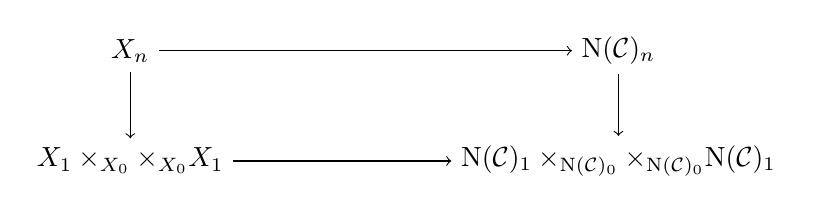
\begin{tikzpicture}
  \node (a) at (0,0) {$X_n$};
  \node (b) at (6.2,0) {$\mathrm{N}(\mathcal{C})_n$};
  \node (c) at (0,-1.4) {$X_1 \times_{X_0} \dotsm \times_{X_0} X_1$};
  \node (d) at (6.2,-1.4) {$\mathrm{N}(\mathcal{C})_1 \times_{\mathrm{N}(\mathcal{C})_0} \dotsm \times_{\mathrm{N}(\mathcal{C})_0} \mathrm{N}(\mathcal{C})_1$};
  \draw[->] (a) -- (b);
  \draw[->] (a) -- (c);
  \draw[->] (b) -- (d);
  \draw[->] (c) -- (d);
\end{tikzpicture}
\end{center}
  其中竖直映射是双射，而下面的纤维积是对\trSource{}映射与\trTarget{}映射作的，且两侧各有 $n$ 个因子。
\end{enumerate}
由 (a)，下面的映射是双射，故上面的水平映射也是双射。这表明映射 $X \to \mathrm{N}(\mathcal{C})$
是单纯集的同构，即 (2) $\Rightarrow$ (3) 得证。

接下来，我们对 $n$ 作归纳证明 (1) $\Rightarrow$ (2)。当 $n = 2$ 时这是清楚的，因为
$2$-\trSpine{}恰是内 $2$-角。于是我们可以假定：对一切严格小于 $n$ 的 $k$，映射 $I^k \to X$
都能唯一提升为 $\Delta^k \to X$；并考虑一个映射 $I^n \to X$，我们希望证明它唯一地扩
张到 $\Delta^n$。我们将证明它对某个 $0 \le j \le n$ 唯一地扩张到 $\Lambda^n_j$，然
后用 (1) 推出断言。我们首先观察到，$I^n \cap \Delta^{n\setminus\{n\}}$ 恰是这个\trSimplex{}的%
\trSpine{} $I^{n-1}$，同样地，$I^n \cap \Delta^{n\setminus\{0\}}$ 也是\trSpine{}。于是，由归纳
假设，对 $\varepsilon = 0, n$，存在唯一的映射 $\Delta^{n\setminus\{\varepsilon\}} \to X$
把从\trSpine{}到 $X$ 的那个映射扩张出来。由于这两个面的交由
$\Delta^{n\setminus\{0,n\}}$ 给出，而它又与\trSpine{}交出一个更小的\trSpine{}，由归纳假设，这两个扩
张在这个交上一致。
于是，我们得到一个映射
\[
I^n \cup \Delta^{n\setminus\{0\}} \cup \Delta^{n\setminus\{n\}} =
\Delta^{n\setminus\{0\}} \cup \Delta^{n\setminus\{n\}} \to X
\]
其中的并是在 $\Delta^n$ 中取的。我们断言，存在到并
\[
\Delta^{n\setminus\{0\}} \cup \Delta^{n\setminus\{n\}} \cup
\Delta^{n\setminus\{1\}}
\]
的唯一扩张。

为此，我们断言 $\Delta^{n\setminus\{0\}} \cup \Delta^{n\setminus\{n\}}$ 包含
$\Delta^{n\setminus\{1\}}$ 的\trSpine{}：从 $i$ 到 $i+1$ 的边（$2 \le i \le n-1$）全部落在
$\Delta^{n\setminus\{0\}}$ 中，而由 $n \ge 3$，从 $0$ 到 $2$ 的边落在
$\Delta^{n\setminus\{n\}}$ 中。于是，存在唯一一个映射 $\Delta^{n\setminus\{1\}} \to X$
在\trSpine{}上扩张这个映射。剩下要证的是，这个映射与所给映射在
\[
\bigl(\Delta^{n\setminus\{0\}} \cup \Delta^{n\setminus\{n\}}\bigr) \cap
\Delta^{n\setminus\{1\}} =
\Delta^{n\setminus\{0,1\}} \cup \Delta^{n\setminus\{1,n\}}
\]
之上一致。

在这两个\trSimplex{}上，映射由其在\trSpine{}上的限制确定，断言即得。归纳地，我们发现所论的映射存在
唯一的扩张成为映射 $\Lambda^n_{n-1} \to X$。由假设 (1)，这个映射现在可以唯一地扩张到
$\Delta^n$。

为了看出 (2) $\Rightarrow$ (1)，我们考虑一个扩张问题 $\beta\colon \Lambda^n_i \to X$，
要证明它唯一地扩张到 $\Delta^n$。显然可以假设 $n \ge 3$，因为 $I^2 = \Lambda^2_1$。
由假设 (2) 与\cref{ex:spine-horn-boundary-inclusions}，存在一个包含映射 $I^n \to \Lambda^n_i$，于是我们可以考虑限制后的
扩张问题。由假设 (2)，这个问题可唯一求解，从而我们得到映射 $\alpha\colon \Delta^n \to X$。
这个映射又可以限制到 $\Lambda^n_i$ 上，我们要证明所得的映射正是 $\beta$。为
此，我们可以把这个映射限制到 $\Lambda^n_i$ 的各面上，即限制到诸
$\Delta^{n\setminus\{j\}}$（$j \neq i$）的并上。易见
\[
\alpha|_{\Delta^{n\setminus\{0\}}} = \beta|_{\Delta^{n\setminus\{0\}}},
\]
因为该\trSimplex{}的\trSpine{}由大\trSpine{}的一个子集给出，而且按其定义 $\alpha|_{I^n} = \beta|_{I^n}$。对
\[
\alpha|_{\Delta^{n\setminus\{n\}}} = \beta|_{\Delta^{n\setminus\{n\}}},
\]
亦然，只要 $\beta$ 在那里有定义。我们需要在 $j \neq 0, n$ 的假设下证明
\[
\alpha|_{\Delta^{n\setminus\{j\}}} = \beta|_{\Delta^{n\setminus\{j\}}}.
\]
为此，我们证明 $\alpha|_{\Delta_{\{j-1,j+1\}}} = \beta|_{\Delta_{\{j-1,j+1\}}}$（同样
，\trSpine{}的所有其余边都已包含在大\trSpine{}之中）。由于 $n \ge 3$，这条边含于
$\Delta^{n\setminus\{\varepsilon\}}$，其中 $\varepsilon$ 为 $0$ 或 $1$。然后我们便
可归纳得知，这确定了来自 $\Lambda^n_i$ 的映射，证明完成。
\end{proof}
事实上，可以说得略多一点：

\begin{lemma}\label{lem:lifting-nerves}
若 $n \ge 4$，$0 \le j \le n$，且 $\mathcal{C}$ 是一个\trCategory{}，则每个提升问题
\begin{center}
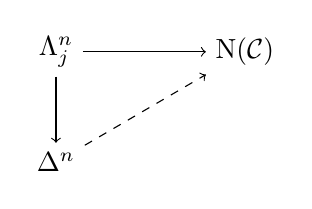
\begin{tikzpicture}
  \node (l) at (0,0) {$\Lambda^n_j$};
  \node (x) at (2.4,0) {$\mathrm{N}(\mathcal{C})$};
  \node (d) at (0,-1.4) {$\Delta^n$};
  \draw[->] (l) -- (x);
  \draw[->] (l) -- (d);
  \draw[->, dashed] (d) -- (x);
\end{tikzpicture}
\end{center}
都可被唯一求解。
\end{lemma}

\begin{proof}
「范畴的神经是 $2$-余\trSkeleton{}的」是\cref{ex:nerve-2-coskeletal} 的内容；我们还将在推论 1.2.21 中给出另一个论
证。于是，只需回忆：对 $n \ge 4$ 与一切 $0 \le j \le n$，
$\mathrm{sk}_2(\Lambda^n_j) \to \mathrm{sk}_2(\Delta^2)$
是同构。\footnote{译注：原书此处作 $\mathrm{sk}_2(\Delta^2)$；按上下文疑应为
$\mathrm{sk}_2(\Delta^n)$。}
\end{proof}

\begin{lemma}\label{lem:nerve-kan-iff-groupoid}
\trCategory{} $\mathcal{C}$ 的\trNerve{}是\trKanComplex{}，当且仅当 $\mathcal{C}$ 是\trGroupoid{}。
\end{lemma}

\begin{proof}
在\cref{lem:nerve-kan-groupoid}中，我们已经见过「$\mathrm{N}(\mathcal{C})$ 是%
\trKanComplex{}蕴含 $\mathcal{C}$ 是\trGroupoid{}」这一方向。现在需要证明另一方向。于是设
$\mathcal{C}$ 是\trGroupoid{}，我们来证明 $\mathrm{N}(\mathcal{C})$ 是\trKanComplex{}。由
\cref{thm:spine-horn-nerve}我们已经知道，可以（唯一地）提升所有内\trHorn{}以及所有维
数大于等于 $4$ 的\trHorn{}。因此，只需证明可以提升外 $2$-角与外 $3$-角。通过转到相
反范畴，只需证明每个扩张问题
\begin{center}
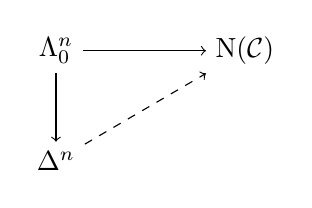
\begin{tikzpicture}
  \node (l) at (0,0) {$\Lambda^n_0$};
  \node (x) at (2.4,0) {$\mathrm{N}(\mathcal{C})$};
  \node (d) at (0,-1.4) {$\Delta^n$};
  \draw[->] (l) -- (x);
  \draw[->] (l) -- (d);
  \draw[->, dashed] (d) -- (x);
\end{tikzpicture}
\end{center}
对 $n = 2, 3$ 都有（唯一的）解。当 $n = 2$ 时，这样的映射由两个映射 $f\colon x \to y$
与 $g\colon x \to z$ 给出；此时我们可以为另一条边选取 $f \circ g^{-1}$。为了对左
外 $3$-角证明断言，我们考虑沿\trSpine{}的限制，得到三个可合成的映射 $f$、$g$ 与 $h$。我们发
现，到 $\Delta^3$ 的扩张存在，恰好当边 $\Delta_{\{1,3\}} \to \Lambda^3_0 \to \mathcal{C}$
由合成 $hg$ 给出时。考虑 $2$-\trSimplex{} $\Delta_{\{0,1,3\}} \to \Lambda^3_0 \to \mathcal{C}$，
我们发现这条边满足「与 $f$ 作预合成给出 $hgf$」这一条件。由于 $f$
是同构，断言得证。
\end{proof}
